\label{fig:prob}
\begin{center}
\begin{figure*}[h]
\begin{center}
\begin{minipage}{0.49\textwidth}
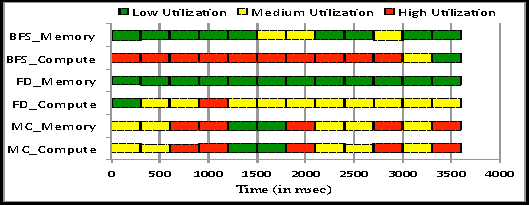
\includegraphics[width=\textwidth, height=3.5cm]{cloud-workload}
\end{minipage}
\begin{minipage}{0.49\textwidth}
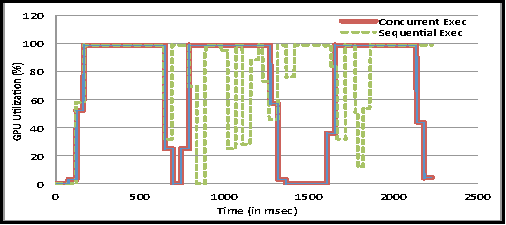
\includegraphics[width=\textwidth, height=3.5cm]{GPU-utilization}
\end{minipage}
\caption{\small a) Compute and memory characteristic of various GPU-based cloud
applications.  b) GPU utilization of Monte Carlo requests following exponential
distribution of request arrival with sequential vs. concurrent execution.}
\label{fig:cloud}
\end{center}	
\end{figure*}
\end{center}
\section{Motivation and Challenges}
\subsection{Scheduling Crisis in GPU Multitenancy}
Current programming models continue to treat GPUs as devices chosen by applications. There are several issues with the consequent programmer-defined selection of target GPUs. First, applications running on a multi-GPU node may compete for the same GPU, thus not able to leverage availability of multiple on-node GPU accelerators and leading to the serialization of GPU requests that otherwise could have been served in parallel. We define such conflicts as \textit{static collisions }between applications’ GPU requests. Second, since applications are unaware of each other’s GPU usage, e.g., their relative GPU intensities, they cannot assess the performance implications of sharing a single GPU. We define this as a \textit{character collision} between the requests from two or more applications sharing a GPU. Both static and character collisions become even more critical when nodes have heterogeneous GPUs with differing capabilities in terms of their compute, memory capacities, and bandwidths. The importance of collisions is underlined by the fact that most cloud applications driven by end user requests vary substantially in their compute and memory characteristics and therefore, have difficulties in fully utilizing both the compute engines and memory capacities of GPUs. We demonstrate this in Figure~\ref{fig:cloud}a., with cloud applications deployed using the CloudBench infrastructure, for exponentially distributed request arrivals. The color-coding in the figure indicates the levels of compute and memory utilization of the applications, varying from heavily utilized (red \textgreater   90\%) to under-utilized (green \textless   10\%). Some of these applications are compute intensive, such as graph algorithm Breadth First Search (BFS), some are memory intensive – financial algorithm Monte Carlo (MC), and some exhibit average utilization levels, like OPENCV face detection (FD). Note that frequent GPU idle intervals occur even for efficient GPU codes like Monte Carlo. Another issue with current GPU programming models is that although each GPU can internally contain thousands of cores, application uses it as a single SIMD engine, which means that the multiple GPU contexts created by host threads can share a GPU only over time, but not in space. CUDA 4.0 addresses this problem by allowing multiple threads within a single host process to share the same GPU context, but GPU utilization could be improved further with true GPU multi-tenancy. We demonstrate this opportunity by manually dispatching multiple sets of independent Monte Carlo requests, again following an exponential distribution of inter-arrival times, over different CUDA Streams from the same GPU context. Figure~\ref{fig:cloud}b. shows GPU usage peak and idle periods to be much more uniform compared to their sequential execution. This is because keeping a single GPU context avoids context switching overhead and this eliminates unnecessary GPU idling during context switching (the ‘glitches’ in the figure), as in the case of independent sets of web requests driving their execution.

The illustrative examples above motivate key properties of the GPU scheduler to achieve effective multi-tenancy in GPU-based servers: (1) load balancing is needed to avoid static collisions, (2) device-level scheduling must be cognizant of character collisions and provide such feedback to the load balancer, (3) additional functionality is needed to achieve resource management goals like fairness, high throughput, etc., and (4) there should be system-level support for reducing GPU core idling when some application’s context cannot fully utilize a single GPU.

\begin{table}[h]
%\begin{tabular}{p{3.5cm} p{2.5cm} p{2.5cm} p{2.5cm}}
\begin{tabular}{cccc}
\hline
{\footnotesize\bf Graphs} & {\footnotesize\bf X-Stream (ms)} & {\footnotesize\bf CuSha (ms)} & {\footnotesize\bf Speedup}\\ 
 \hline
{\footnotesize ak2010} &  {\footnotesize 215.155} & {\footnotesize 7.75 } & {\footnotesize 28x}\\   

{\footnotesize belgium\textunderscore osm} &  {\footnotesize 2695.88} & {\footnotesize 791.30} & {\footnotesize 3x}\\   

{\footnotesize coAuthorsDBLP} &  {\footnotesize 1275} & {\footnotesize 11.55} & {\footnotesize 110x}\\   

{\footnotesize delaunay\textunderscore n13} &  {\footnotesize 80.89} & {\footnotesize 5.18} & {\footnotesize 16x}\\   

{\footnotesize kron\textunderscore g500-logn20} &  {\footnotesize 46550.7} & {\footnotesize 119.82} & {\footnotesize 389x}\\   

{\footnotesize webbase-1M} &  {\footnotesize 3909.12} & {\footnotesize 13.52} & {\footnotesize 290x}\\   
  \hline
\end{tabular}
\caption{\footnotesize Performance comparision between two state-of-the-art
graph processing approaches. X-Stream runs on a 16 core Xeon
E5-2670 CPU with 32GB memory. CuSha runs on a NVIDIA
K20c Kepler GPU with 4.8 GB memory.}
\vspace{-1.5ex}
\label{tab:hw}
\end{table}
 
\subsection{Why Graph Analytics Using GPUs ?}
The high compute power and multi-level parallelism provided by the SIMT (Single Instruction Multiple Threads) architectures of GPGPUs present opportunities for accelerating many graph algorithms. Table ~\ref{tab:hw} shows the performance comparison between two state-of-the-art graph analytics processing the BFS algorithm: X-Stream~\cite{xstream} for CPUs and CuSha~\cite{cusha} for in-memory GPU processing. Significant performance speedups are observed from using the GPU. For instance, graph kron\_g500-logn20 processed by CuSha on a commercial K20c Kepler GPU (4.8GB memory) achieves 390x speedup over X-Stream on a 16 core Xeon E5-2670 CPU (32 GB memory). This clearly motivates to exploit the extreme parallelism offered by thousands of cores of GPUs for real-world graph analytics. 
